\section{Risk Demonstration - Sub-Saharan Africa}

\section{Description}
A demonstrative test has been created in which economic losses due 
to damage in residential buildings are estimated for the Grater Accra 
district, in Ghana. This region is affected by low seismicity, with 
expected ground acceleration of $1 ms^{-2}$ for a probability of 
exceedance of 10\% in 50 years. The required OpenQuake input files
have been compiled, and a brief description of each component is 
provided below. 

\section{Exposure Model}
The Ghana Statistical Service [1] carries out Housing Census every
10 years which provides sufficient information for the development 
of an accurate exposure model. However, for the sake of simplicity,
this model created for this exercise was developed based on a simplified
approach in which population spatial distribution is used to extrapolate 
building value. In order to do so, it is fundamental to comprehend in
which building typologies does the Ghanaian population reside. 

According to Kishor et al. (2010), in urban areas, approximately 
82\% of the population live in rubble stone masonry buildings and 
17\% in mud wall houses. The remaining 1\% is distributed in wood
and other informal types of construction. Applying these percentages
to a spatial distribution of population dataset such as GRUMP [2], 
it is possible to obtain the number of people in each building 
typology in an evenly spaced grid. Then, these results are combined
with the average living area per person and the replacement cost 
per unit of area for Ghana (taken from the Ghana Statistical Service),
to derive economic value of each building typology (in EUR), 
following the same evenly spaced grid. The outcome of this 
exercise is illustrated in Figure \ref{fig:accra_exposure}.

\begin{figure}[htb]
	\centering
		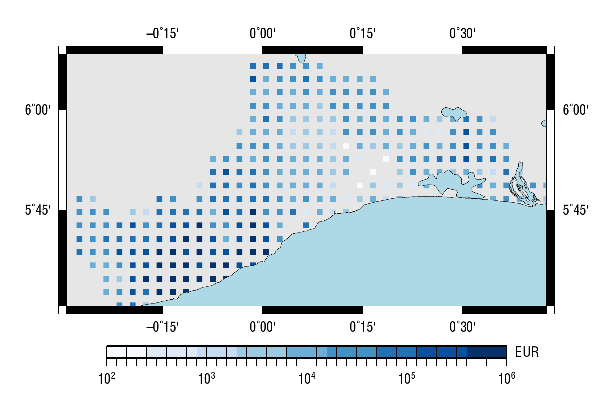
\includegraphics[height=6.5cm, keepaspectratio=true]{./figures/exposure.eps}
	\caption{Exposure Model for the Great Accra District}
	\label{fig:accra_exposure}
\end{figure}

\section{Vulnerability Model}

Three building typologies were considered for this example: wooden 
frame building (W), rubble stone masonry (RS) and mud walls buildings 
(MW). There is very little information about the seismic vulnerability 
about such typologies, so in order to create a vulnerability model for
this demo, vulnerability from similar building typologies as well as 
damage data from the Cambridge Architectural Research database were 
used, to derive the vulnerability model depicted in Figure 
\ref{fig:vulnerability}. 

\begin{figure}[htb]
	\centering
		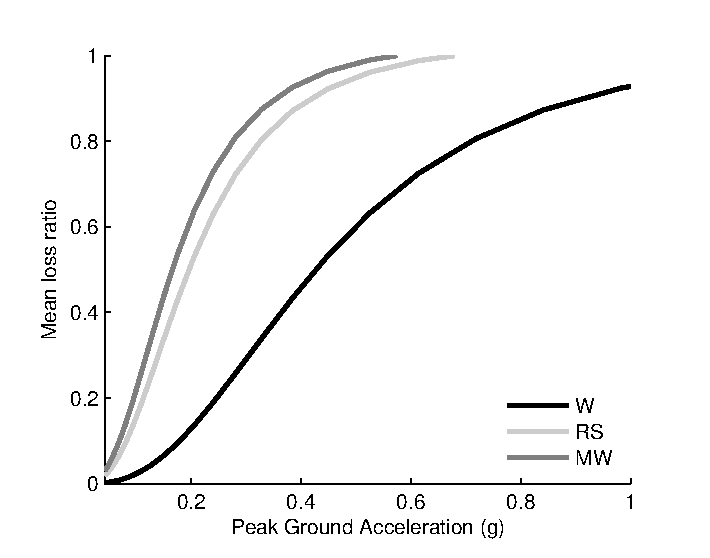
\includegraphics{./figures/vulnerability.eps}
	\caption{Vulnerability Model for Building Typologies in Ghana}
	\label{fig:vulnerability}
\end{figure}

Due to the large uncertainty about the structural behaviour of these
types of structures, a coefficient of variation of 30\% was assumed 
for each loss ratio.

\subsection{Rupture Model}

In order to select a reasonable magnitude for an event in Ghana, 
a set of past events were studied, and it was concluded that a
magnitude of 6.5 ($M_W$) would be acceptable. Considering this
magnitude and the Wells and Coppersmith relationship, a rupture
length of approximately 30 km was estimated. The distribution of 
faults in the territory around Ghana was evaluated a fault capable
of triggering such event was selected (see Figure \ref{fig:rupture}). 
For this demo, the ground motion prediction equation for Stable 
Continent tectonic region (Toro et al, 2002) was chosen. 

\begin{figure}[htb]
	\centering
		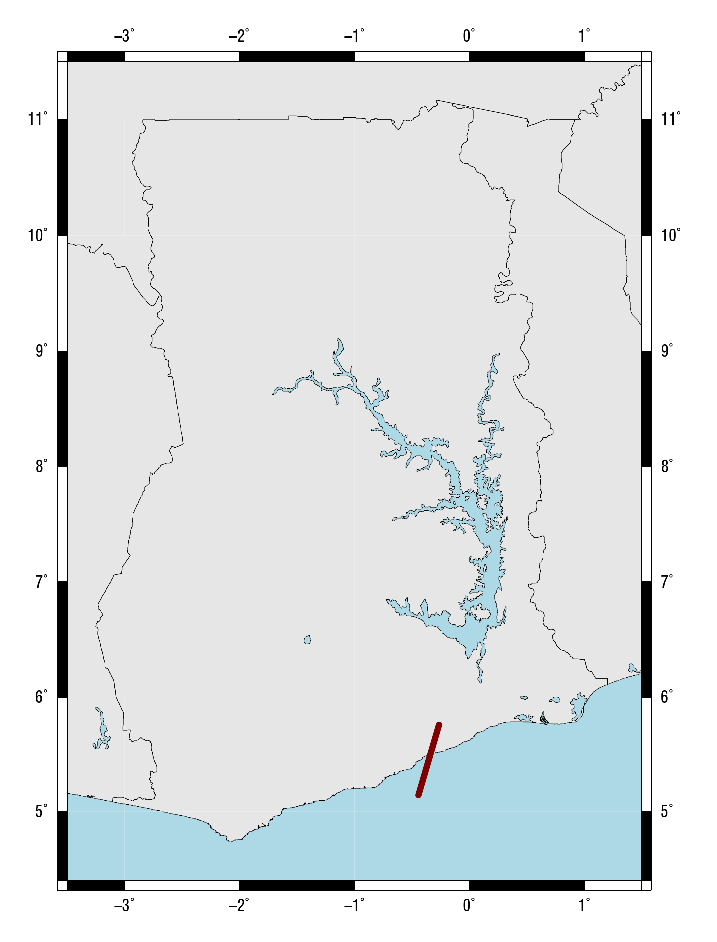
\includegraphics{./figures/rupture.eps}
	\caption{Rupture trace (in red) for a deterministic event in Accra}
	\label{fig:rupture}
\end{figure}
